\chapter{Introduction}
\label{sec:Introduction}
% Thesis statement. 

%Particle colliders allow us to study quantum chromodynamics (QCD), 

% Study nuclear physics
One of the major goals of high-energy physics is to study quantum chromodynamics (QCD), the theory of the strong nuclear force which describes the interactions between quarks and gluons.
Quarks and gluons are the building blocks of atomic matter; every proton has two up quarks and a down quark, and every neutron has two down quarks and an up quark. 
Gluons mediate the interactions between those quarks.
Despite their prominance, these particles are never observed in isolation under standard terristrial conditions.
They are always found together in the form of hadrons, which are particles such as protons and pions that have two or three quarks bound together.
This phenomenon, the fact the quarks are not normally observed in isolation, is called confinement.
However, at sufficiently high density and temperature, it is possible to have a medium that is too hot for hadrons.
Instead, the quarks and gluons exist freely, and their collective behavior exhibits fluidlike properties \cite{Heinz:2005zg}.
This medium is called the quark-gluon plasma (QGP).
By studying the QGP, as well as the conditions that exist after the QGP dissipates, physicists can get more insight into the strong nuclear force.

Modern particle accelerators create conditions under which the QGP can exist for a short time \cite{Heinz:2000bk}.
This is primarily done via the collision of heavy ions such as $\ce{^197 \mathrm{Au}}$ and $\ce{^208 \mathrm{Pb}}$.
At energies seen by the Large Hadron Collider (LHC), the ions travel at nearly the speed of light ($c = 3 * 10^8 \mathrm{\frac{m}{s}}$), and they have center of mass energies per nucleon on the order of tera electron Volts (TeV).
The collisions of these ions can produce a hot, dense medium from which thousands of particles are emitted \cite{Aamodt:2010cz}.
This medium (the QGP and subsequent hadronic phase) has several names, such as "interaction region" or "particle-emitting source", though it is colloquially called a fireball.
The collision, the medium, and the subsequently emitted and measured particles are collectively known as an event. 

\begin{figure}[hbt]
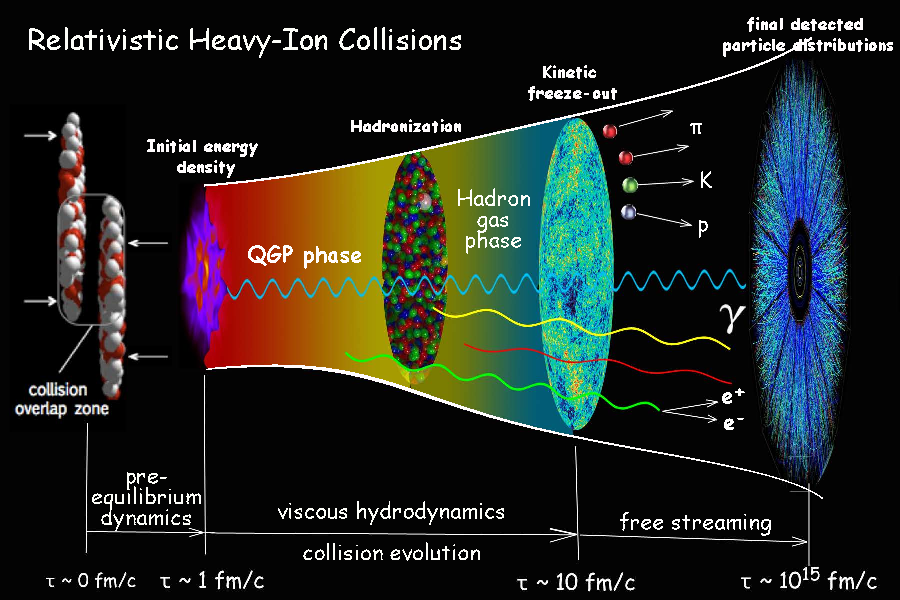
\includegraphics[width=36pc]{Figures/BorrowedFigures/HeavyIonEvolution.pdf}
\caption[Evolution of a heavy ion collision]{Evolution of a heavy ion collision \cite{Shen:2015msa}. 
Two ions collide and leave behind a medium of high energy density. 
After about 1 fm/$c$ ($\sim 10^{-23}$ s), the medium thermalizes as a plasma of deconfined quarks and gluons. 
After a few fm/$c$, the quarks and gluons cool down and hadronize into pions, kaons, and many other particles. These hadrons scatter off each other few more fm/$c$, until the become so dilute that they free-stream to a detector.}
\label{fig:HeavyIonEvolution}
\end{figure}

Figure \ref{fig:HeavyIonEvolution} shows a cartoon of a heavy ion collision.
It is suspected that the QGP exists for only a few moments after the collision of these ions, on time scales of about a few fm/$c$ (femtometers per speed of light, with 1 fm/$c$ = $10^{-15} \mathrm{m}/c \sim 10^{-23}$ seconds).
Over time the plasma expands and cools, and eventually the quarks and gluons combine to form hadrons, a process called hadronization.
In the subsequent hadronic phase, the hadrons scatter off each other in an elaborate billiard ball game, with particles near the edge of the expanding fireball having the possibility to free-stream to the detector.
Eventually, the source becomes dilute enough that the inter-particle scatterings die off. This occurs on time scales on the order of 10 fm/$c$ \cite{BraunMunzinger:2007zz}.
While people often speak of a singular kinetic freezeout time (the time when the rescatterings cease), in actuality particles are emitted at varying rates throughout the lifetime of the fireball.

Heavy-ion physics programs such as ALICE (A Large Ion Collider Experiment) seek to study the evolution of these fireballs.
The field tries to answer questions such as "When does hadronization occur?", "What equations of state describe the evolution of the interaction region?", "What interactions are occuring between particles during during this evolution?", and "What is the size and shape of the medium at kinetic freezeout?".
A number of models have been developed to probe these questions and others \cite{Werner:2010aa,Karpenko:2012yf,Bozek:2012qs,Schenke:2009gb}, and experimental results help refine these models.

Generally speaking, collision models have three main components: initial conditions describing the shape and energy density of the source; a theory describing how the system evolves over time; and the final result of collision, namely a description of the particles that are emitted including their momenta, emission time, etc.
%Collider experiments have been designed so as to simplify assumptions about the initial conditions of fireballs.
Collider experiments have been designed to simplify assumptions about the initial conditions of fireballs, and to measure their asymptotic state.
$\ce{^197 \mathrm{Au}}$ and $\ce{^208 \mathrm{Pb}}$ ions are used since these particles have a spherical symmetry to their nuclear structure that gives the fireballs a relatively simple initial geometry.
Particle collider experiments provide insight into the final state of collisions by measuring the final momenta of particles produced in millions of events.

% Heavy-ion models act as a bridge...
%In the last 15 years, the Relativistic Heavy Ion Collider (RHIC) has performed Au--Au and U--U collisions, and the Large Hadron Collider (LHC) has done Pb-Pb collisions.

%By looking at the final-state information of large ensembles of collisions and making various model assumptions about the initial conditions and evolution, it is possible to work backward to obtain a better grasp of what happens in the early stages of the collisions.
%To answer many of the above questions, it is often necessary to look at this final-state information and work backwards.

Beyond simply measuring asymptotic particle momenta, collider experiments can use an assortment of analysis techniques to probe various facets of the fireball evolution.
These techniques include flow analysis \cite{Aamodt:2010pa,Heinz:2013th}, the study of particle spectra \cite{Aamodt:2010cz}, and an interferometry technique known as femtoscopy \cite{Aamodt:2011mr,Lisa:2005dd}.
In the following sections, we'll give an overview of the LHC and the ALICE detector.
We'll then give a short description of a few of the ongoing physics programs.
Finally, we'll move on to the main topic of this thesis: femtoscopy.

\section{Particle collider experiments}

\subsection{The Large Hadron Collider}
\label{sec:TheLHC}

\begin{figure}[hbt]
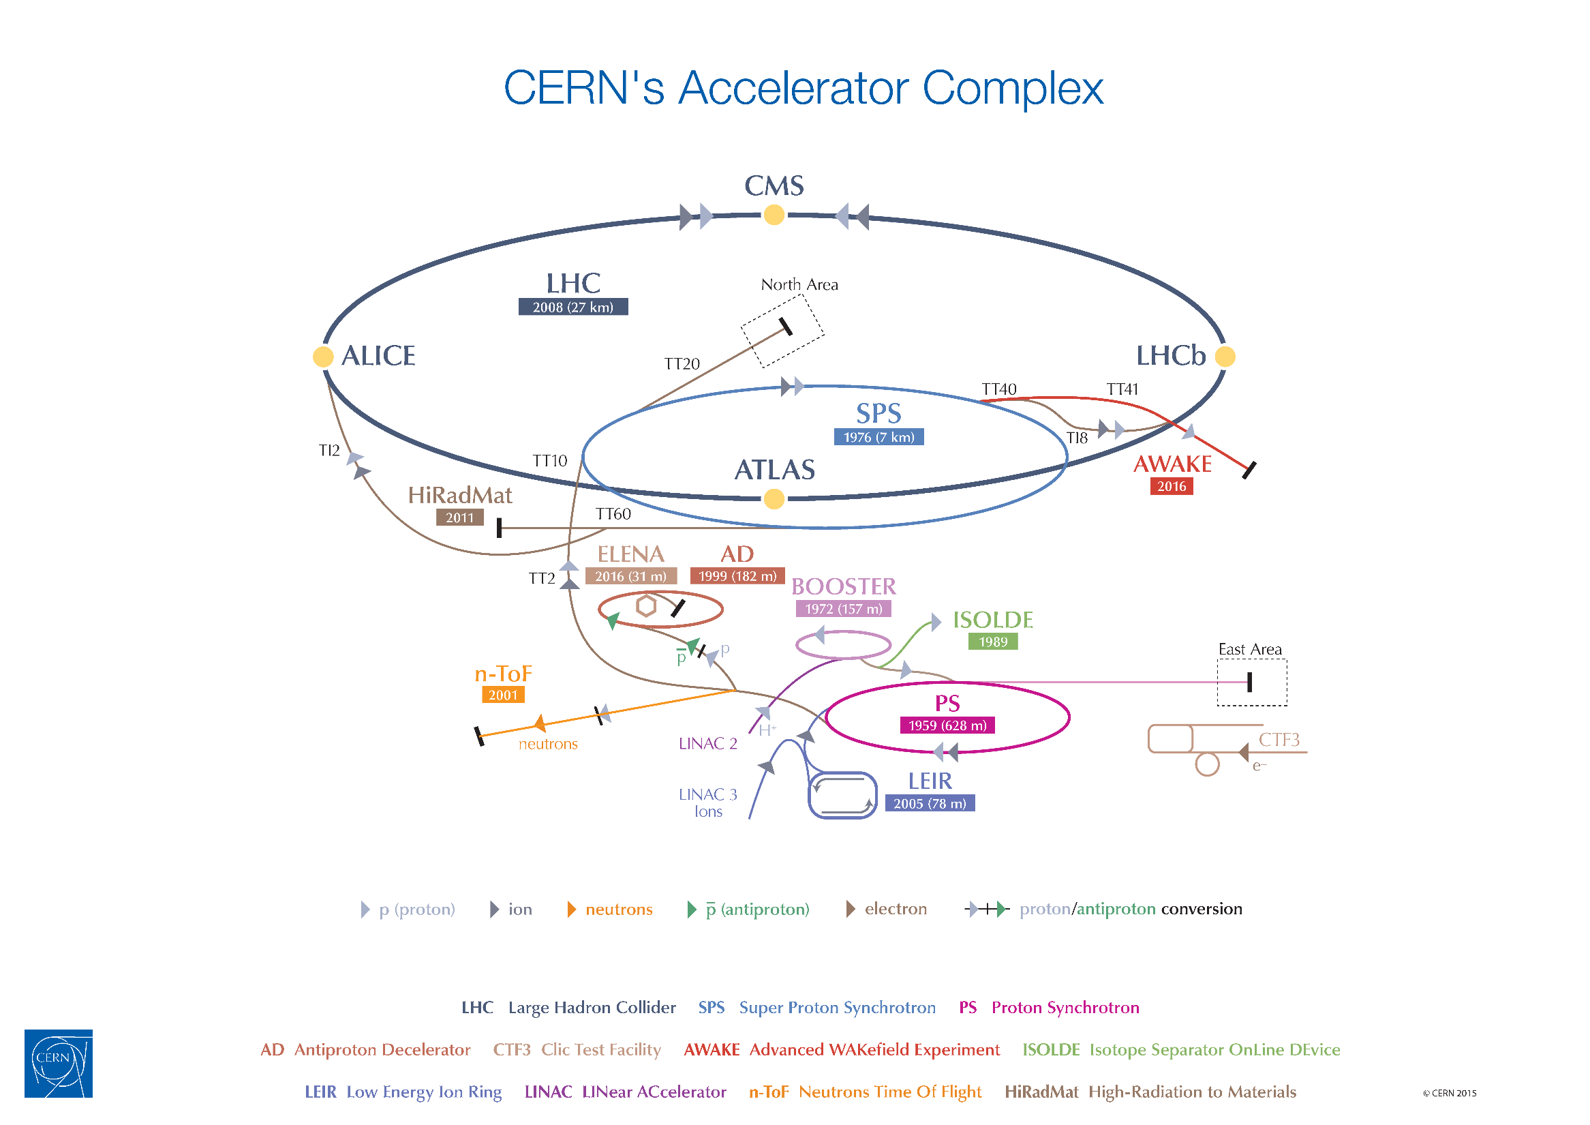
\includegraphics[width=36pc]{Figures/BorrowedFigures/CERNComplex.png}
\caption[Schematic of the LHC]{A schematic of the Large Hadron Collider \cite{EspaceCERN}. 
Proton and/or Pb ion beams go through a series of accelarators before being injected into the LHC. Beams travel in both directions around the LHC, and the two beams are only allowed to collide at the four experiments: ALICE, ATLAS, LHC-b, and CMS.}
\label{fig:CERNComplex}
\end{figure}

ALICE is one of several experiments at the Large Hadron Collider.
The LHC itself is part of the European Organization  for Nuclear Research (CERN, from the French \it Conseil Europ\'een pour la Recherche Nucl\'eaire\rm).
CERN is near Geneva, Switzerland, and the 27 km ring of the LHC lies partly in France and partly in Switzerland.
%There are several detectors built around the ring.

The LHC is literally built upon previous successful experiments. 
In order to get protons and ions traveling at very nearly the speed of light, they are sent through a series of increasingly powerful accelerators, each of which was a state of the art machine for particle physics in its day.
Figure \ref{fig:CERNComplex} shows a diagram of the LHC and the accelerators that feed into it.
Particles are injected into the LHC ring in bunches of up to $10^{11}$ particles, with bunches traveling in both clockwise and counterclockwise directions around the ring \cite{Lefevre:1092437}.
The bunches are spaced a few nanoseconds apart.
There are thousands of bunches per beam in proton-proton mode, while Pb-Pb mode has hundreds.
Those bunches are steered around the ring with magnets as strong at 8 Tesla.
The two beams are only allowed to intersect at four points, the four major LHC experiments: ALICE, LHC-b, CMS, ATLAS.
At these intersection points, there can be millions or even hundreds of millions of proton-proton collisions per second.
Ions have collision rates in the thousands.
 
\subsection{The ALICE detector}
\label{sec:ALICEDetector}

 
\begin{figure}[hbt]
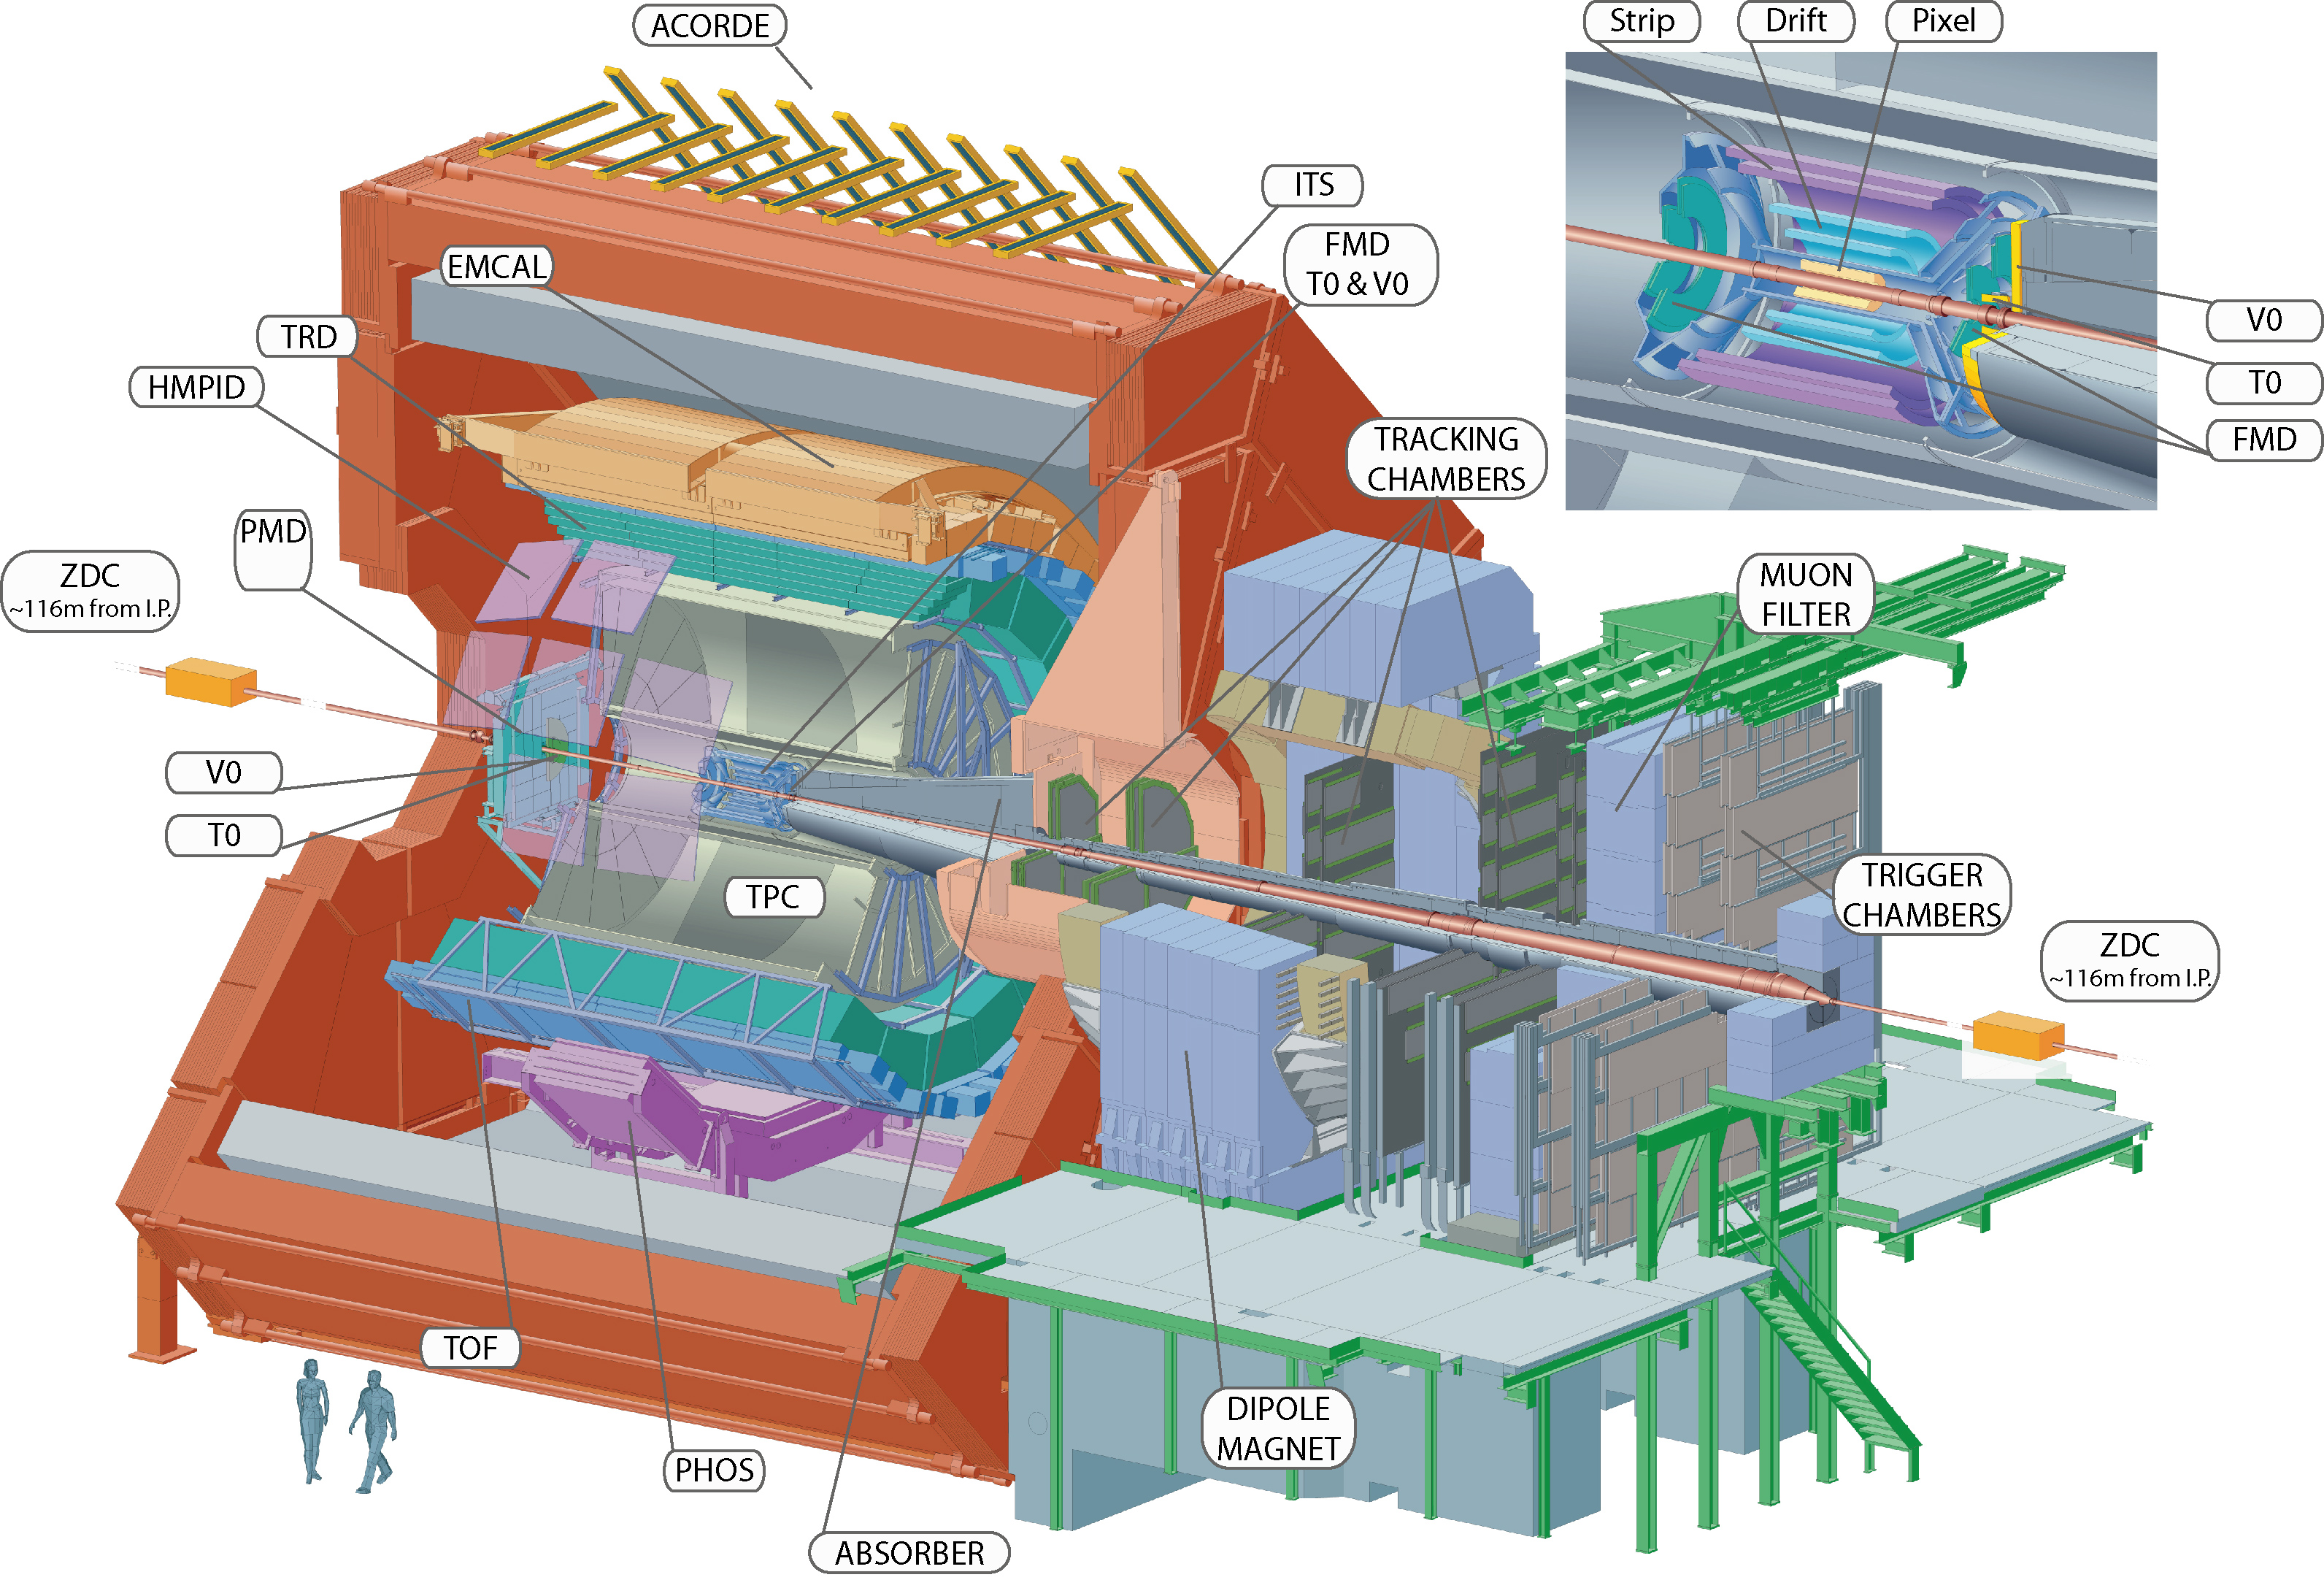
\includegraphics[width=36pc]{Figures/BorrowedFigures/ALICEDetector.jpg}
\caption[Cartoon of the ALICE detector]{A cartoon of the ALICE detector \cite{Aamodt:2008zz}.}
\label{fig:ALICEDetector}
\end{figure}
%The primary research focus of the ALICE detector is to measure and analyze heavy-ion collisions.
Figure \ref{fig:ALICEDetector} shows a cartoon of the ALICE detector.
The main barrel of the detector is 14.1 m long and 15.8 m in diameter. The outer layer (shown in red in the cartoon), is an 0.5 T solenoidal magnet.
The two beams are steered such that most collision events occur within 10 cm of the longitudinal center of the detector (i.e. along the beam axis), and within about a cm of the radial center.

The ALICE detector is composed of many subdetectors \cite{Aamodt:2008zz}, several of which are designed to monitor the trajectories of charged particles that pass through them.
These reconstructed trajectories are called tracks.
The inner most detector is the Inner Tracking System (ITS), which provides full azimuthal coverage with a radial range of 3.9 cm to 43 cm.
The ITS consists of 6 layers of silicon detectors: two Silicon Pixel Detectors, two Silicon Drift Detectors, and two Silicon Strip Detectors.
The ITS serves multiple purposes.
The spatial resolution of the various layers ranges from tens to hundreds of $\mu$m.
With hundreds (p-p) or thousands (Pb-Pb) of particles produced in each collision, the ITS is able to reconstruct the position of the collision with a resolution better than 100 $\mu$m.
The collision location is called the primary vertex, as nearly all the reconstructed particles trace back to it.
The ITS also provides position tracking and particle identification (PID) for low-momentum particles via $\frac{\mathrm{d}E}{\mathrm{d}x}$ measurement \cite{Jackson:1998nia}.
Finally, the tracking resolution of the ITS allows it to identify secondary vertices, the locations where hyperons (baryons containing a strange quark) and various heavy mesons decay into charged particles.

The next detector is the Time Projection Chamber (TPC) \cite{ALICE:2014qrd}, which spans $r=85$ cm to $r=250$ cm.
The TPC is a 5 m long barrel full of a 90:10:5 mixture of Ne, CO$_2$, and N$_2$ gas.
The barrel is divided in half longitudinally by a 100 kV electrode, and there are readout electronics on either end.
When a charged particle passes through the TPC, it ionizes the gas in its wake.
The electric field then drives the electron clouds toward the readout electronics.
These clouds quickly reach their max drift velocity of 2.7 cm/$\mu$s (27 km/s). 
The position of the track can thus be determined by the length of time it takes for the ionized gas to reach the readout chamber.
The 0.5 T magnetic field causes the track's trajectory to bend, and the particle's momentum can be determined by the curvature of the track.
The TPC therefore is able to determine the 3D position of the track throughout the TPC with mm precision, the momentum of the charged particle, and its d$E$/d$x$ value.
This is the main tracking system of the ALICE detector, and it can provide PID information for particles with momentum up to $\sim 1$ GeV/$c$.

\begin{figure}[hbt]
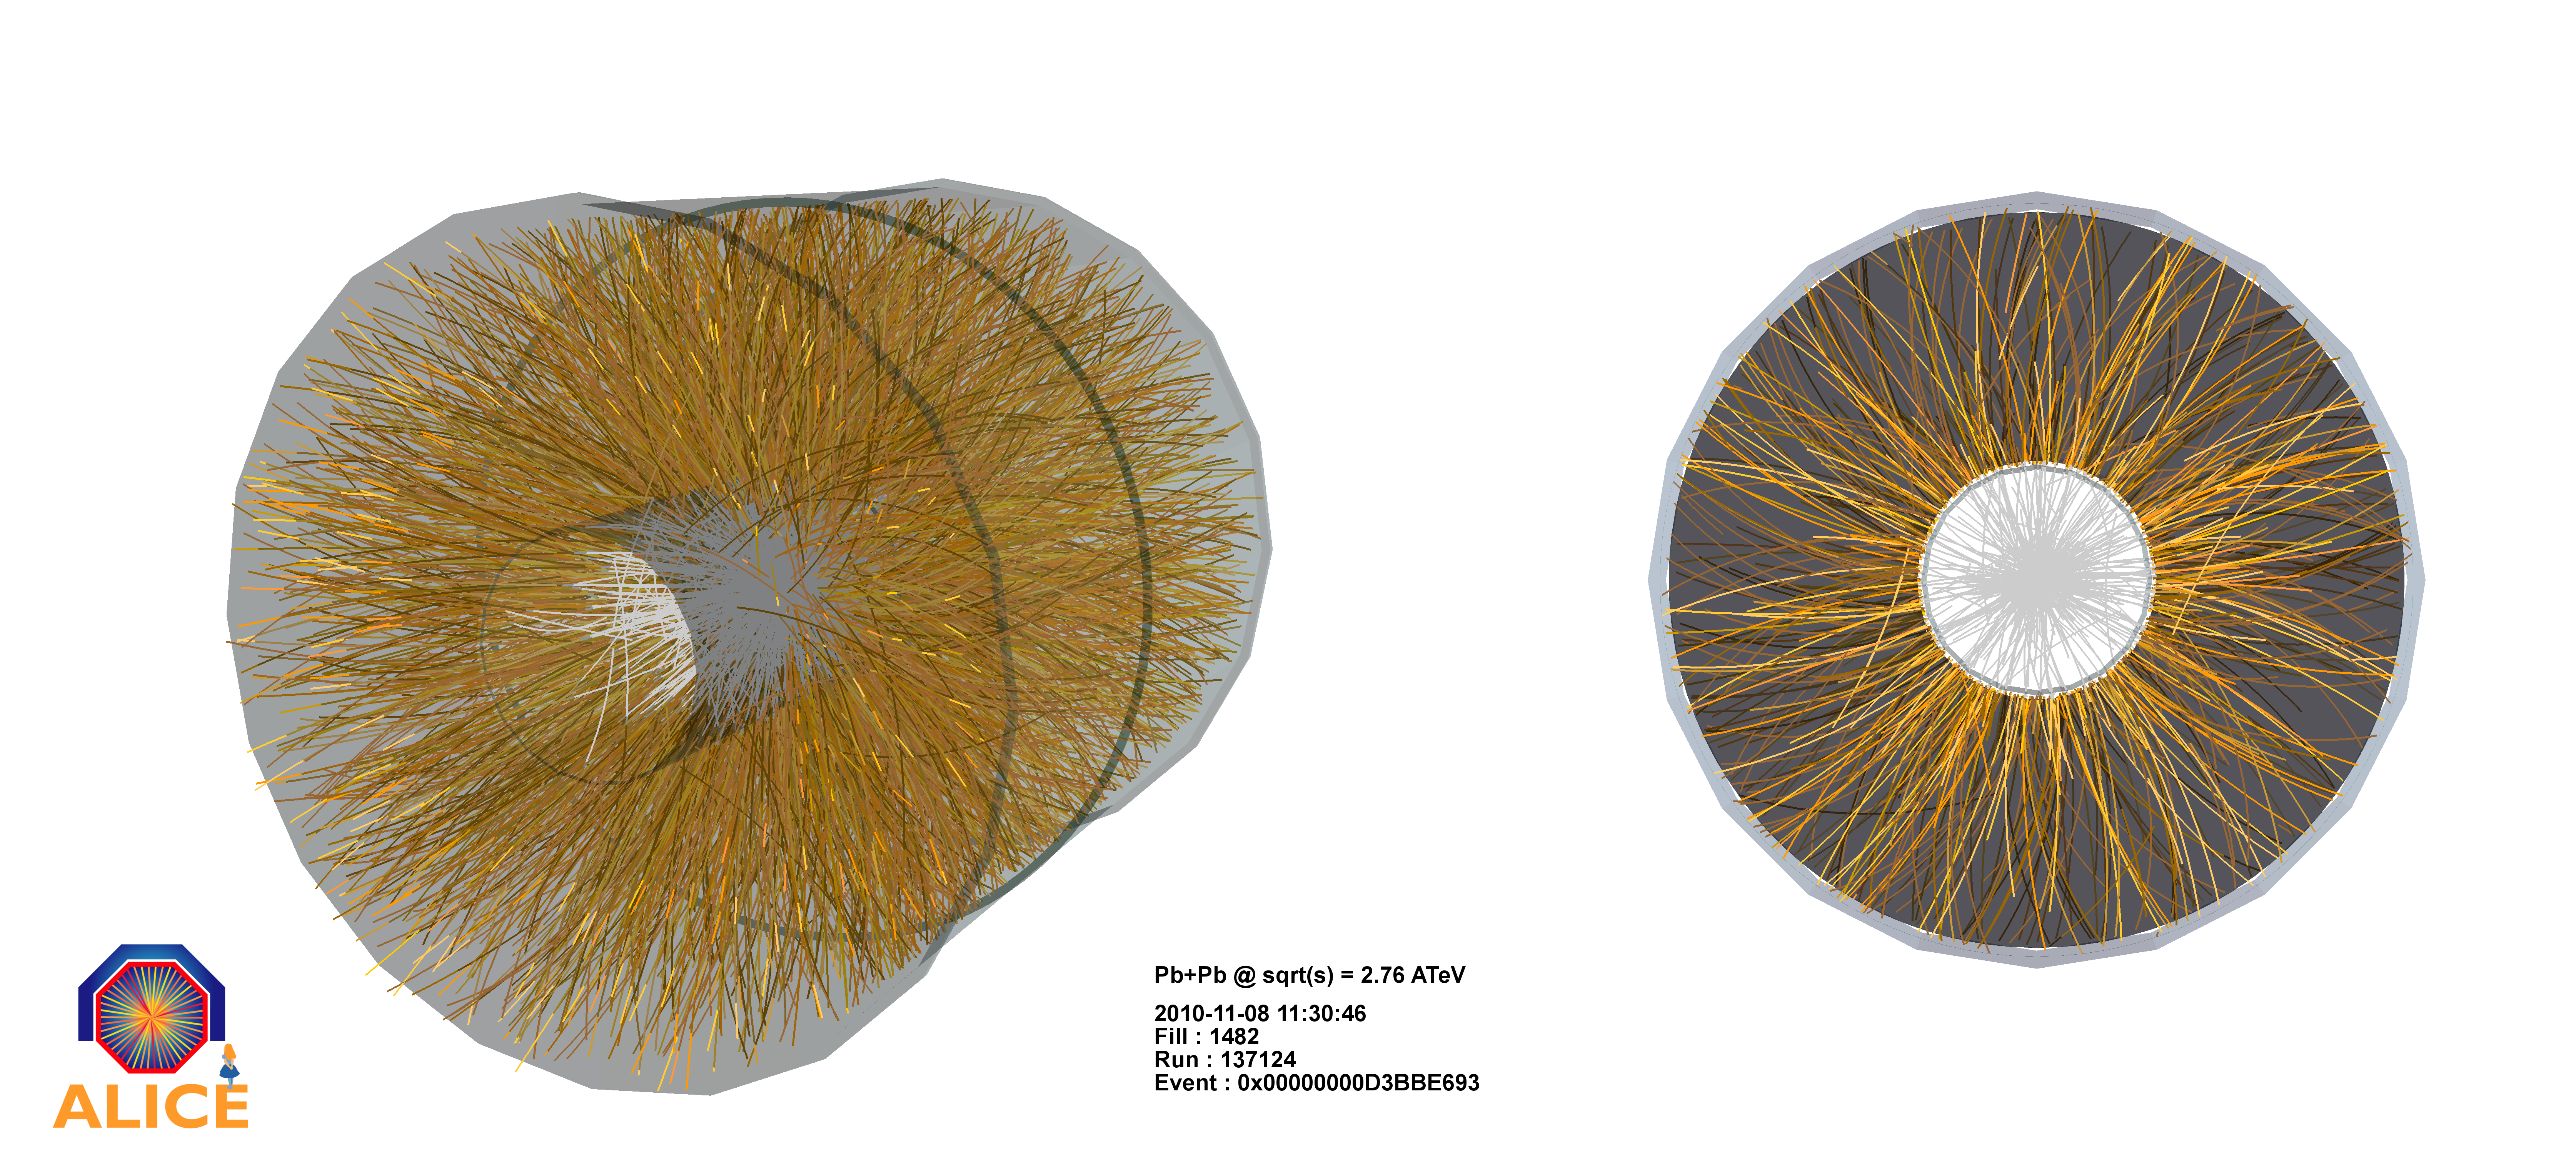
\includegraphics[width=36pc]{Figures/BorrowedFigures/ExampleCollision.png}
\caption[Example of a Pb-Pb collision]{An example of a Pb-Pb collision measured at the ALICE detector.
Charged particles traveling through the detector leave behind tracks that the detector can measured, each of which is depicted by a colored line.
The white region in the center of the detector is the Inner Tracking System, while the surrounding grey region is the Time Projection Chamber.
Tracks measured by the ITS are grey, while tracks found by the TPC are yellow.
Combined tracking information from both detectors is used to improve the momentum resolution of each track.
}
\label{fig:ExampleCollision}
\end{figure}
Figure \ref{fig:ExampleCollision} shows a Pb-Pb collision recorded in the first run of the LHC.
The tracking by the ITS is shown in white, while tracking from the TPC is yellow.
The TPC can provide quality tracking information for ion events with thousands of charged particles, but it has the drawback of being a slow detector compared to the ITS.
The maximum drift time of a track is about 90 $\mu$s, so if two or more events occur within that window their tracking information can overlap.
This is called event pile-up.
The TPC can isolate and record central Pb-Pb events (events with head-on collisions) at a rate of 300 Hz and p-p events at a rate of 1 kHz.

The Time-Of-Flight (TOF) detector is a 20 cm thick shell around the TPC.
In conjunction with the T0 detector which determines the timing of the initial collision, the TOF can measure the time it takes a particle to reach it.
With this information and momentum information from other tracking detectors, the mass of the particle can be determined.
The TOF can successfully distinguish between particles with momentum as low as 0.5 GeV/$c$ up to 3-4 GeV/$c$, depending on the particle, and it essential for PID of particles above the 1 GeV/$c$ limit of the TPC. 

The T0, VZERO, and Zero Degree Calorimeter (ZDC) detectors provide event triggering for the ALICE detector.
Event-triggering detectors monitor activity in the beam collision area, and they inform the detector when to record data.
The ALICE detector therefore does not need to record information for every interaction, including interactions from the occasional cosmic rays striking the detector or the beam striking ambient gas.
Instead, it can use event triggers to selectively record events that appear relevant to the designated research goals of the ALICE collaboration.
For example, there may be an interest in central collisions, which produce the most particles.
The primary triggers used by ALICE with Pb-Pb events are minimum bias, semi-central, and central, each of which will be described in the following section.

\subsection{Event characterization}
\label{sec:EventCharacterization}

It is often useful to classify a heavy-ion collision by how central/peripheral (head-on/glancing) the collision is.
Figures \ref{fig:GlauberImpactParameter}, \ref{fig:GlauberCentrality}, and \ref{fig:NpartCentrality} show several ways of quantifying this \cite{Abelev:2013xaa, Aamodt:2010pa}.
One is by impact parameter $b$, which is the distance from the center of one nucleus to the center of the other.
Another is by the total number of participants $N_\mathrm{part}$ --- the nucleons from either ion that interact with nucleons from the other ion.
With 208 nucleons in a Pb nucleus, the maximum number of participants is 416.
A third way of classifying them is by multiplicity (the number of particles produced in each collision), as central collisions tend to produce more particles than peripheral collisions.

While any of these definitions might be useful from a theoretical standpoint, they have varying degrees of usefulness and accessibility in an experimental setting.
Impact parameter, with a scale of femtometers, is inaccessible by experimental measurement.
The number of participants can be estimated using detectors such as the ZDC, which measure the number of spectator nucleons (nucleons that are not participants) on a collision.
And the number of particles is easily quantified; in practice, experiments often use the number of charged particles in an event as a proxy for the total number of particles in the event.
At ALICE, typically only particles found
at mid-pseudorapidity $\abs{\eta} < 0.8$ are used in these estimates, where pseudorapidity is defined as
\begin{equation}
\label{eq:Pseudorapidity}
\eta = \frac{1}{2} \ln \left( \frac{\abs{p} + p_{\mathrm{z}}}{\abs{p} + p_{\mathrm{z}}} \right),
\end{equation}
and $p$ and $p_\mathrm{z}$ are a particle's three-vector momentum and momentum along the beam axis, respectiviely.

\begin{figure}[hbt]
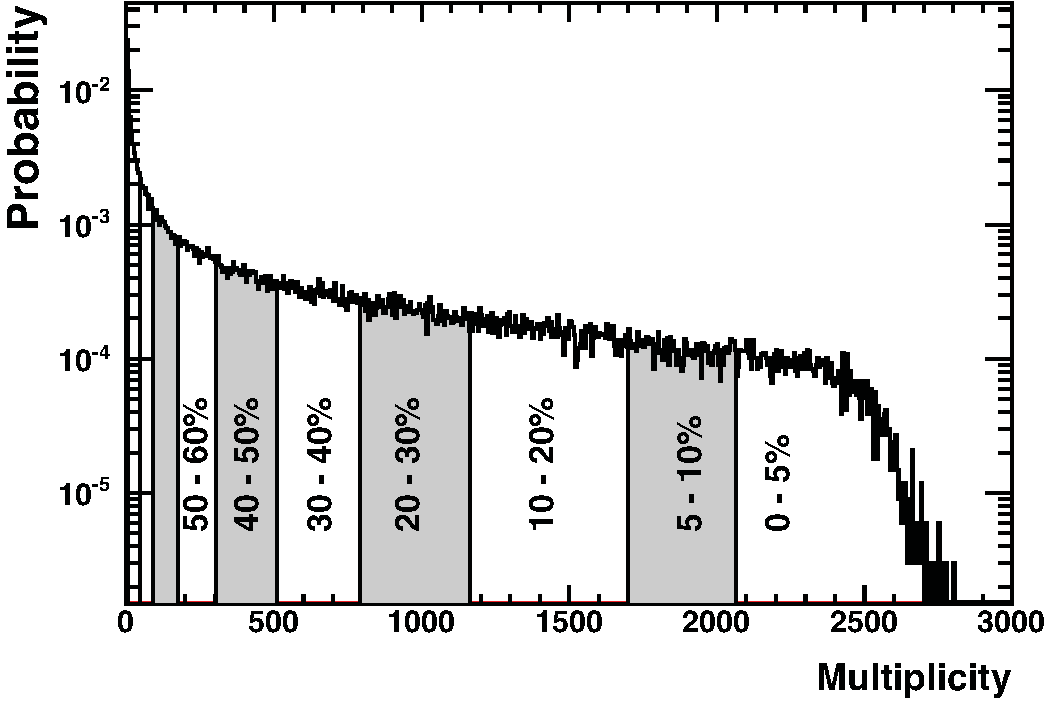
\includegraphics[width=36pc]{Figures/BorrowedFigures/NpartCentrality.pdf}
\caption[Charged-particle multiplicity distribution used for centrality definition]{
Uncorrected charged-particle multiplicity measured by the ALICE TPC at mid-pseudorapidity ($\abs{\eta} < 0.8$) in $\sqrt{s_\mathrm{NN}} = 2.76$ TeV Pb-Pb collisions \cite{Aamodt:2010pa}.
Centrality classes are defined in percentile bins with 0-5\% corresponding to the most central collisions with the largest multiplicities, and 95-100\% corresponding to peripheral collisions with the smallest multiplicities.}
\label{fig:NpartCentrality}
\end{figure}
\begin{figure}[hbt]
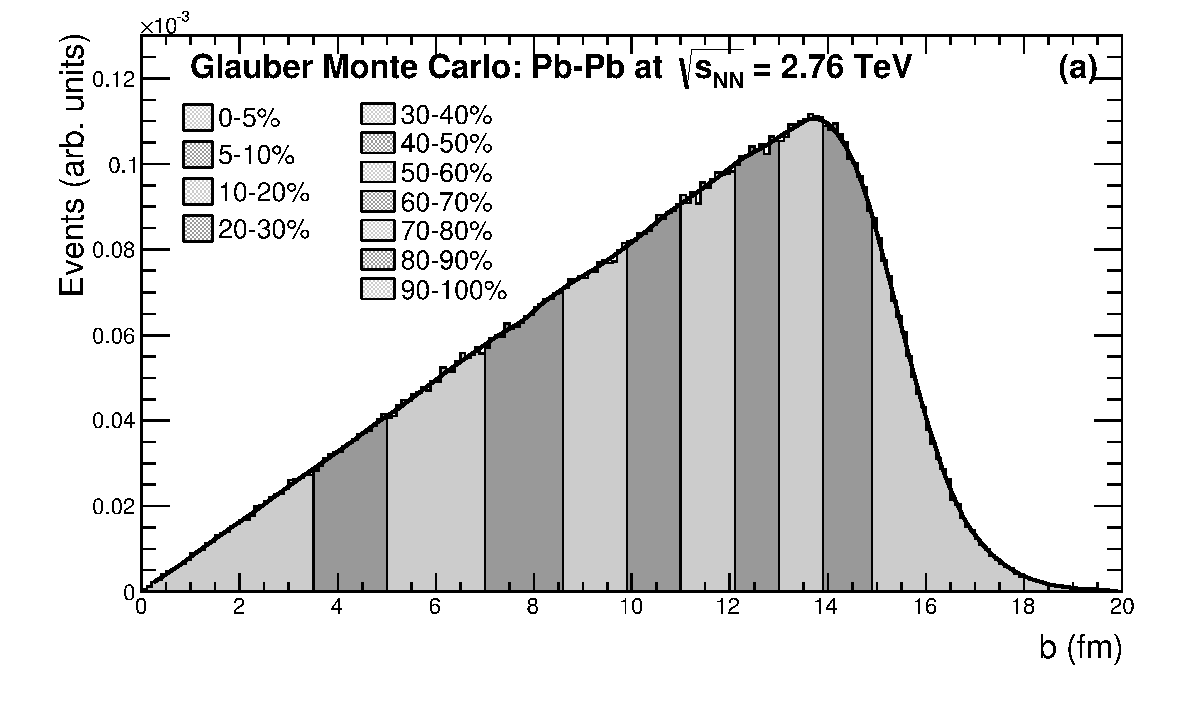
\includegraphics[width=36pc]{Figures/BorrowedFigures/GlauberImpactParameter.pdf}
\caption[Monte Carlo Glauber impact parameter simulation]{Distribution of $\sqrt{s_\mathrm{NN}} = 2.76$ TeV Pb-Pb collision impact parameters $b$ from a Monte Carlo Glauber simulation \cite{Abelev:2013xaa}.
Impact parameter is defined as the distance between the center of one nucleus to the center of the other at the time of the collision.
Bands indicate the impact parameters associated with different centrality classes.
}
\label{fig:GlauberImpactParameter}
\end{figure}
\begin{figure}[hbt]
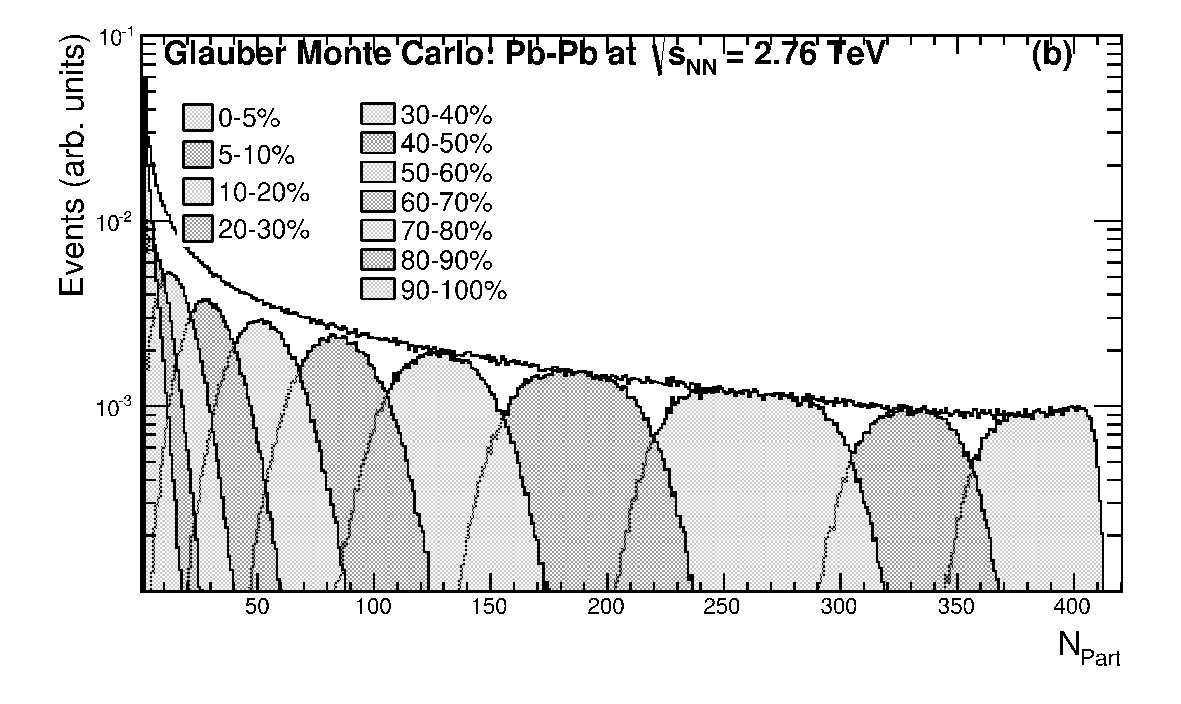
\includegraphics[width=36pc]{Figures/BorrowedFigures/GlauberCentrality.pdf}
\caption[Monte Carlo Glauber number of participants simulation]{A Monte Carlo Glauber simulation of the total number of nucleons involved in $\sqrt{s_\mathrm{NN}} = 2.76$ TeV Pb-Pb collisions \cite{Abelev:2013xaa}.
A nucleon from one ion that interacts with a nucleon from another is called a participant.
In a peripheral collision, each ion only has a handful of participants.
Central collisions may have $\sim 200$ participants per ion.
The estimated participant ranges of the centrality classes are shown.
}
\label{fig:GlauberCentrality}
\end{figure}

To bridge these various ways of classifying collisions, we define centrality classes.
There are a number of ways to calibrate centrality, the most common of which is by ranking events in terms of their multiplicity.
Central collisions (0-10\%) have the highest multiplicity, while peripheral (90\% and above) collisions have the smallest, as seen in Figure \ref{fig:NpartCentrality} \cite{Aamodt:2010pa}.
Centrality can also be mapped onto theoretical calculations of impact parameter (Figure \ref{fig:GlauberImpactParameter}) and $N_\mathrm{part}$ (Figure \ref{fig:GlauberCentrality}) \cite{Abelev:2013xaa}.

Multiplicity estimates from the TPC, along with timing information and other signals from the ZDC and VZERO, provide event triggering and centrality measurements.
The minimum bias trigger records an even sampling of the centrality distribution.
The central trigger records only 0-10\% central events, and the the semi-central trigger records events in the 10-50\% centrality range.

\section{Heavy-ion analyses}

%\subsection{Jet quenching}
\subsection{Flow}
\label{sec:Flow}

\begin{figure}[hbt]
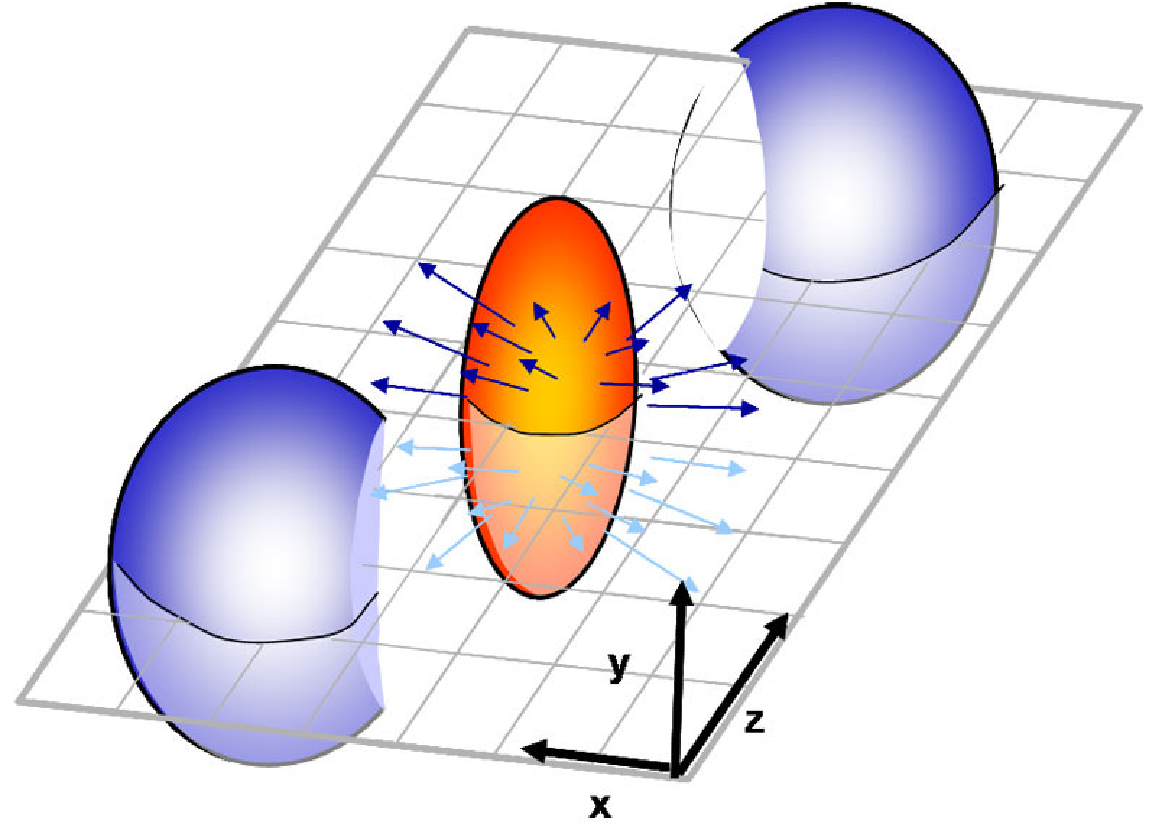
\includegraphics[width=36pc]{Figures/BorrowedFigures/Almond.pdf}
\caption[Non-central collision]{ 
Cartoon of a non-central heavy-ion collision \cite{Rapp:2008qc}.
The blue shapes are the recently-collided ions, while the overlap region of the expanding fireball is orange.
The almond-shaped fireball is taller than it is wide, which results in a larger pressure gradient along the x-axis than along the y-axis.
This pressure gradient causes the fireball to expand more rapidly along the x-axis than along the y-axis.
}
\label{fig:Almond}
\end{figure}
When two ions collide, the topology of their overlap region has a pronounced effect on the momentum distribution of the particles produced in the collision.
Figure \ref{fig:Almond} shows a cartoon of a non-central heavy-ion collision.
At LHC energies, the colliding ions are Lorentz length-contracted by a factor of $\sim 1500$, effectively making them flat disks or pancakes with non-uniform density (more nucleons in the center than towards the edge).
When these two pancakes collide with a non-zero impact parameter, the overlap region of their participant nucleons is roughly almond shaped.
As shown in the figure, the almond-shaped fireball is taller than it is wide.
This creates a larger pressure gradient along the axis of the impact parameter (the short axis) than along the long axis.
This drives a faster expansion along the short axis as the fireball evolves.
In this way, the initial shape of the collision impacts the final momentum distribution of the event, a phenomenon called anisotropic flow.
Using a Fourier decomposition of the the azimuthally-dependent momentum distribution of events, anisotropic flow can be quantified in terms of flow coefficients $v_n$.
Elliptic flow and triangular flow, $v_2$ and $v_3$,  are the most studied coefficients.
Elliptic flow owes much of its existence to the initial spatial anisotropy of the almond-shaped fireball, but triangular flow comes from event-by-event energy density fluctuations in the interaction region.

The study of anisotropic flow helps us understand the initial conditions and the evolution of heavy-ion collisions.
Theorists have had a great deal of success modeling  this evolution, and the evolution of the QGP phase in particular, using relativistic hydrodynamic calculations \cite{Heinz:2013th}.
This has lead some to declare that the quark-gluon plasma is "most perfect fluid" \cite{Heinz:2005zg}, due to its adherence to ideal fluid dynamics.
Nonetheless, viscous effects have been found to have significant effects on the flow coefficients for particles with large transverse (radially outward from the beam axis) momentum $p_\mathrm{T}$.
Flow studies continue to be an important tool in understanding the dynamics of heavy-ion collisions.

\subsection{Spectra}

If the fireball of a heavy-ion collision is in an evolving thermal equilibrium as hydrodynamic models suggest, then it should be possible to quantify the temperature of the fireball at different points in its lifetime.
Some temperature information can be learned from spectral analyses, which measure the number of particles produced in collisions.
There are a few ways to disect spectra.
For each species of particle (e.g.\ $\pi$, K, p), one can look at how many of them are produced on average for a given event.
For a system in thermal equilibrium, the expected number of particles $n_i$ of a particular species in a given energy state $E_i$ follows the distribution
\begin{equation}
\label{eq:ThermalDistribution}
n_i(E_i) = \frac{g_i}{e^{(E_i - \mu_b)/kT} \pm 1}
\end{equation}
where $g_i$ is the degeneracy of the state, $\mu_b$ is the baryochemical potential of the system,  $T$ is the temperature of the system, and the  $+/-$ is for fermions/bosons. 
The baryochemical potential quantifies the baryon-antibaryon asymmetry of the system; $\mu_b = 0$ means that there are equal numbers of baryons and antibaryons.
% citation needed

%One can also look at the momentum distribution of a particular particle species

\begin{figure}[hbtp]
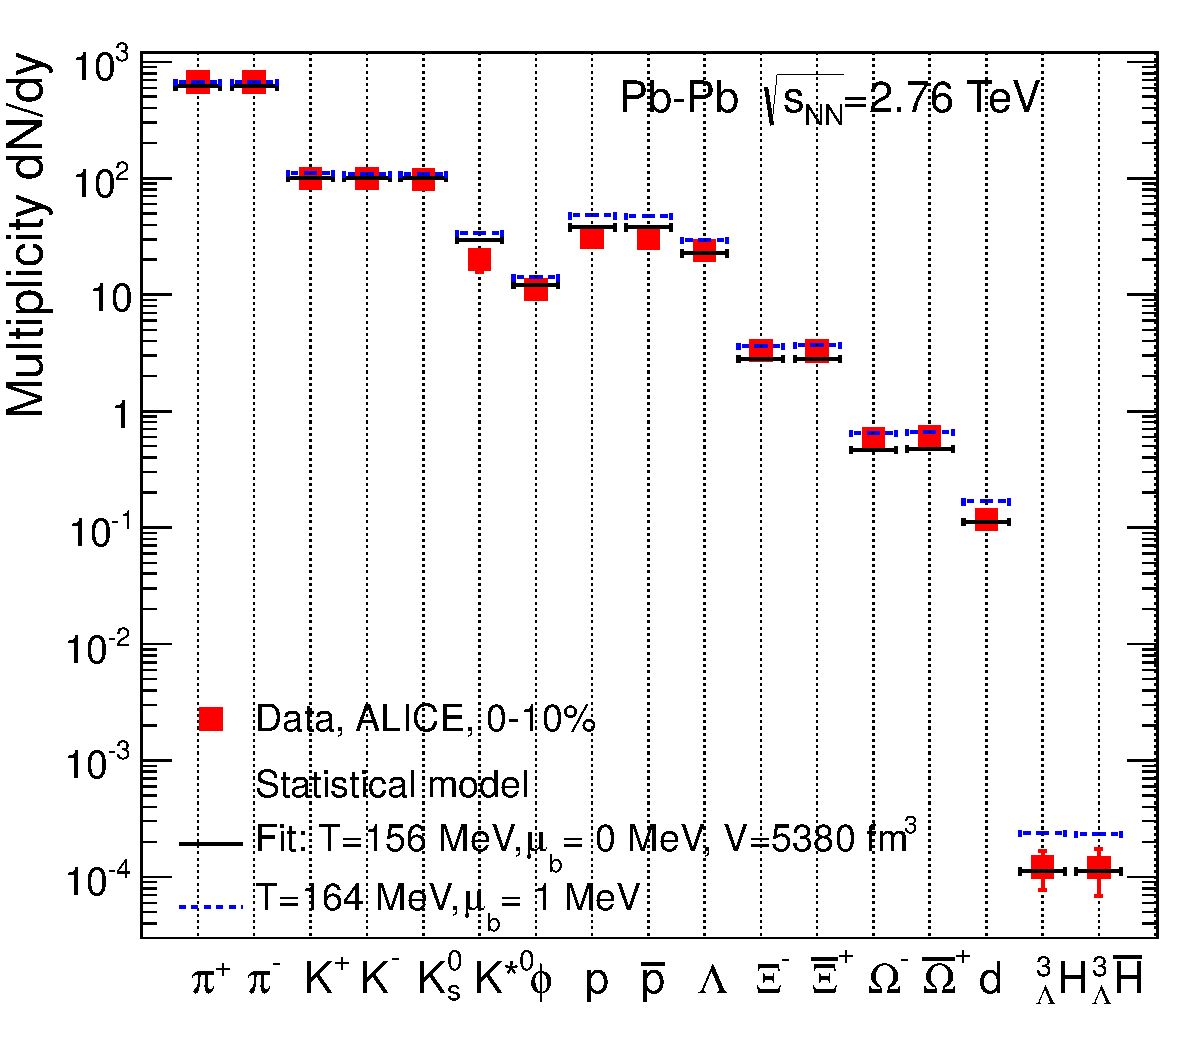
\includegraphics[width=36pc]{Figures/BorrowedFigures/ALICEYieldsThermalFit.pdf}
\caption[Thermal fit of ALICE yields]{Particle yields from central Pb-Pb collisions at ALICE, which are fit with a statistical hadronization model \cite{Stachel:2013zma}. 
The fit suggests that the particle abundances, which mostly appear to obey a thermal distribution, cease to evolve below the temperature $T = 156$ MeV .
The fit also finds that the baryon chemical potential is zero, which means that there is no asymmetry between the matter and antimatter yields of the system. 
}
\label{fig:ThermalYieldFit}
\end{figure}

Figure \ref{fig:ThermalYieldFit} shows particle yields measured in central Pb-Pb collisions at ALICE.
Those yields have been fit with a thermal model \cite{Stachel:2013zma}. 
The fit finds that the baryochemical potential is zero, as one expects at LHC energies.
Most of the particle species appear to obey a thermal distribution for $T = 156$ MeV, which suggests that relative particle yields cease to evolve below that temperature.
That said, the proton and antiproton yields both lie a couple sigma below the thermal value, and studies are ongoing to determine what physics effects might drive these particles out of equilibrium.


\section{Femtoscopy (HBT)}
\label{sec:FemtoHBT}
Hanbury-Brown and Twiss first used two-particle interferometry of photons to measure the angular size of the star Sirius \cite{HanburyBrown:1956bqd}.
Later, it was observed that similar techniques could be employed in a laboratory setting with pions ($\pi$) to characterize the size of particle collisions \cite{Goldhaber:1960sf}.
This process of measuring two-particle correlations for pairs of particles with very similar momentum is often referred to as HBT, after the progenitors of the technique.
HBT was originally used to study photons and later used to look at pions, so it often carries a connotation of Bose-Einstein correlation effects, i.e. the quantum mechanical tendency of identical bosons to exist in the same state. This is in contrast to Fermi-Dirac statistics, wherein identical fermions cannot occupy the same state because of the Pauli exclusion principle.
Modern analyses look at all manner of hadrons, and therefore the correlations might be subject to bosonic, fermionic, or non-identical particle statistics.
In the nuclear physics context, the focus of these analyses is on measuring very small sources, so the more general term \textit{femtoscopy} has come into use.

%\begin{figure}[hbt]
%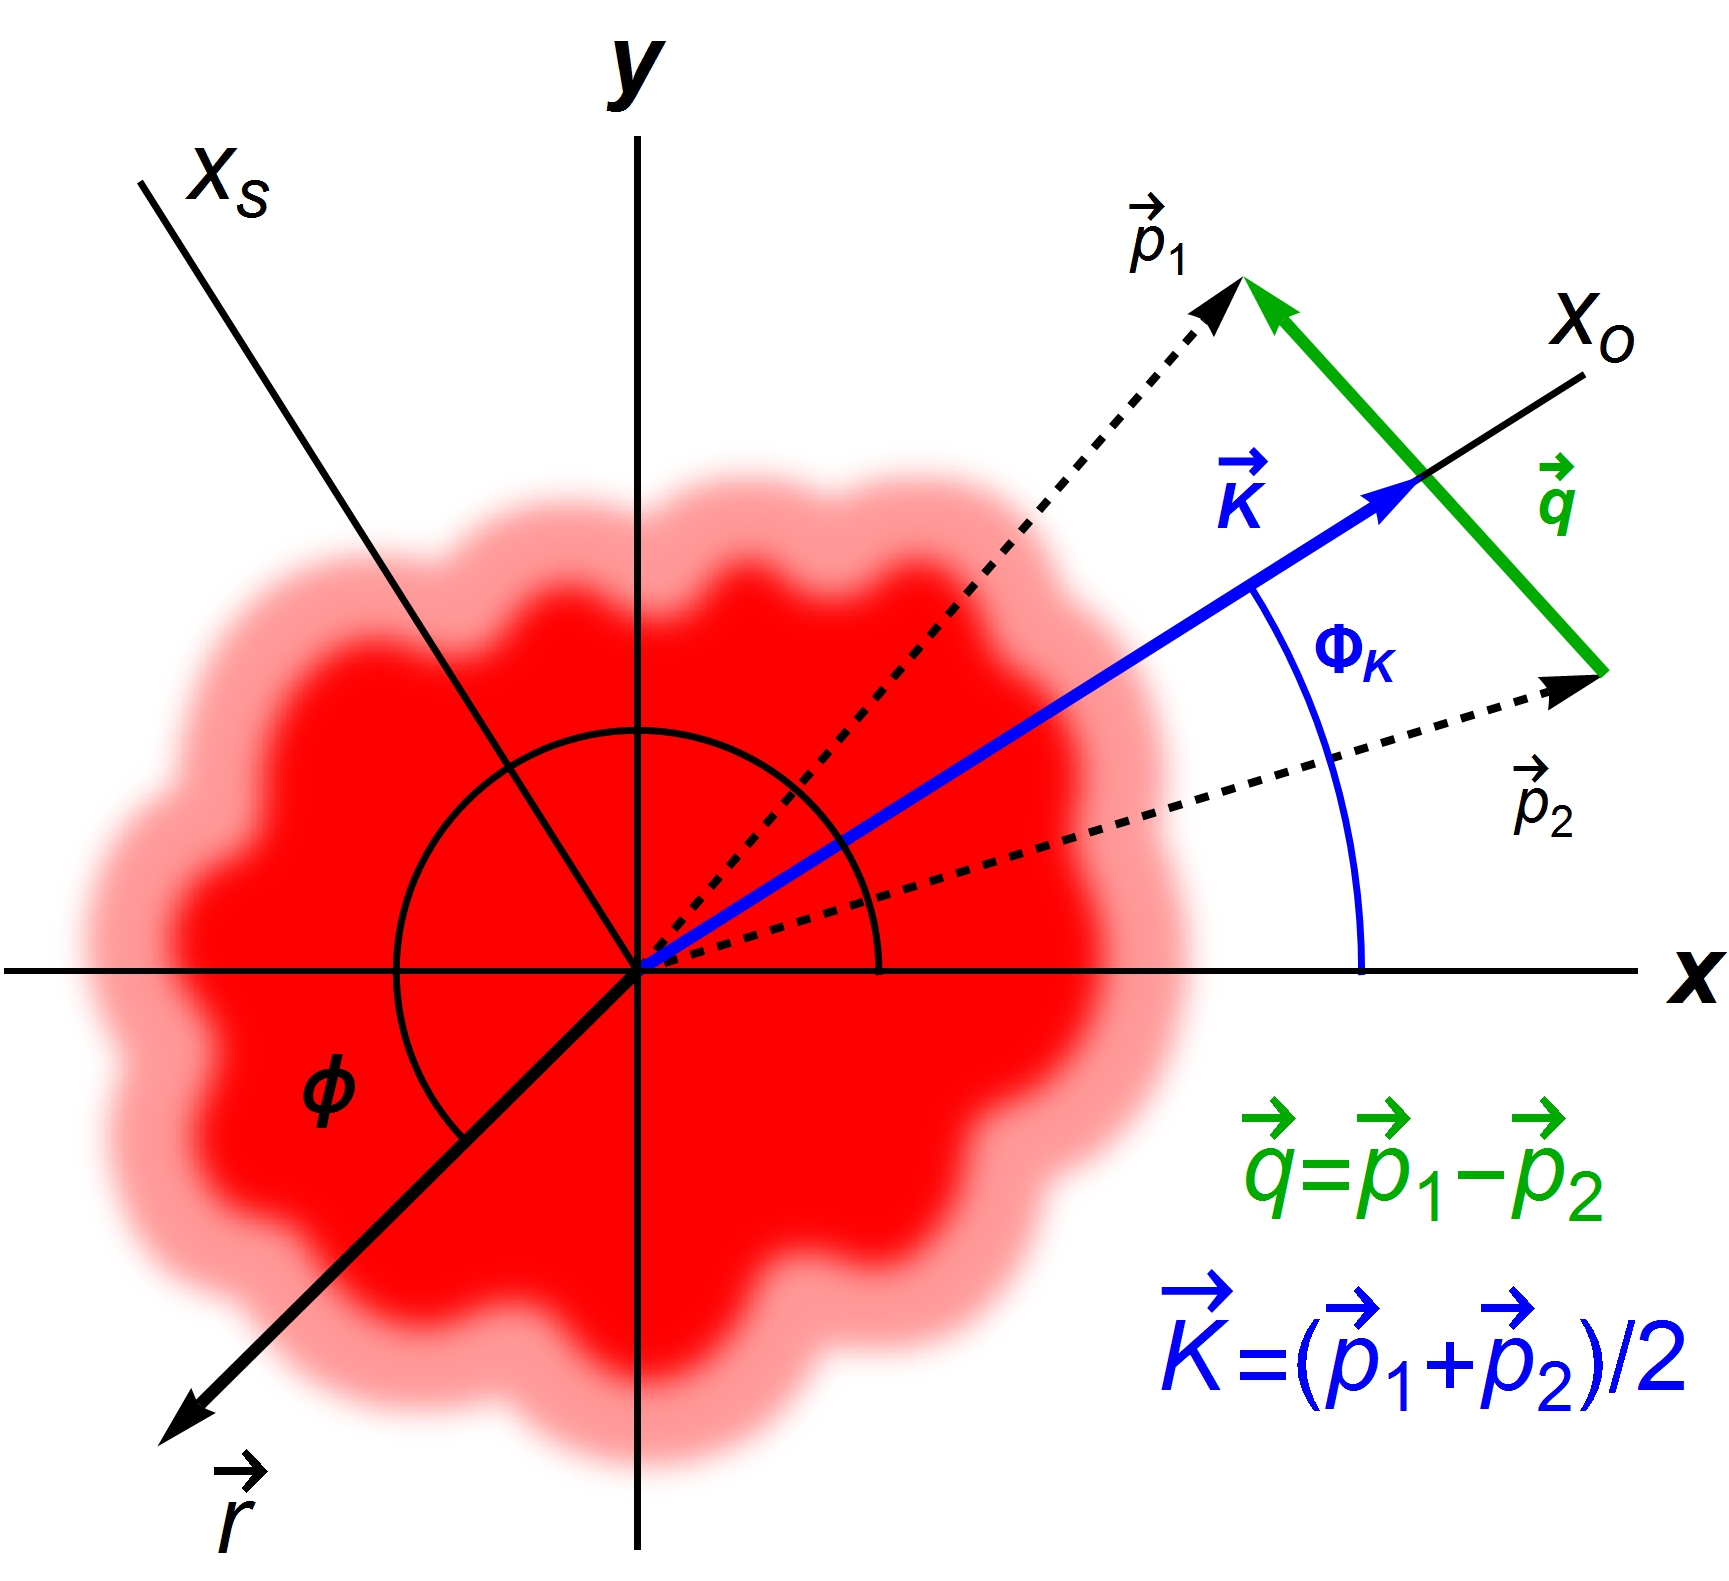
\includegraphics[width=24pc]{Figures/BorrowedFigures/QandK.jpg}
%\caption[Relative momentum]{A cartoon showing the relative momentum $\vec{q} = \vec{p}_1 - \vec{p}_2$ for a pair of particles being emitted from a heavy-ion collision \cite{Plumberg:2016sig}.}
%\label{fig:QandK}
%\end{figure}

Femtoscopic analyses are capable of probing both the two-particle emission function (i.e the size and shape of the source) and the interactions between particles. 
The primary tool of femtoscopy is the correlation function.
A femtoscopic correlation function is constructed by binning the momentum difference $k^\mu = (p_1^\mu - p_2^\mu)/2$ of pairs of particles (this form of $k^\mu$ holds for identical particles; the general form is given in Equation \ref{eq:kmu}).
This is done for both a signal distribution and a background distribution, and the correlation function is the ratio of the two.
With a carefully chosen background distribution, uncorrelated phase space effects are divided out, and the correlation function can reveal correlated physics effects.
Correlation functions are normalized such that a value of unity for a given bin suggests that there are no correlated effects between the particles in that bin.
A value above unity means that some effect is causing an increase of pairs at a given relative momentum, while a value below unity (but never below zero) suggests that some effect is supressing pairs at that relative momentum.
More details on the experimental construction of correlation functions can be found in Section \ref{sec:CorrelationFunctionConstruction}.

As will be discussed in Section \ref{sec:CorrelationFunctionModel}, there is a correlation between the relative position of the particles at their moment of last scattering and their subsequent momentum at freezeout.
The relative position of the particles is described by a two-particle emission function, which is essentially a probability distribution function for finding two particles separated by $\vec{r} = \vec{x}_1 - \vec{x}_2$.
The final state of the particles, including their momenta, depends on the interactions between the particles and is accounted for by the two-particle wave function of the pair.
The correlation function $C_P(k^*)$ is the convolution of the emission function and the wave function:
\begin{equation}
\label{eq:KooninPrattInIntro}
C_P(k^*) =  \int d^3r S_{P} (r) \abs{\Psi(k^*,r)}^2.
\end{equation}
Here $k^* = \sqrt{-k^\mu k_\mu}$ is the magnitude of the relative momentum, $S_P(r)$ is the emission function for pairs of particles with total momentum $\vec{P} = \vec{p}_1 + \vec{p}_2$, and $\Psi(k*,r)$ is the properly symmetrized two-particle wave function of the pair.
The wave function acts to Fourier transform the source function from a relative position space to relative momentum space.
In the following two sections, we'll discuss the source functions and the interactions that make up the wave functions in greater detail.

\subsection{Femtoscopic sources}
\label{sec:FemtoSources}

% chaotic source
%In the context of both astronomy and particle physics, HBT/
Femtoscopy is built on measuring the interference patterns of particles emitted incoherently from a source, be it a star or a heavy-ion collision.
As will be discussed in greater detail in Section \ref{sec:CorrelationFunctionModel}, femtoscopy does not actually measure the size of the full interaction region of a heavy-ion collision at the time of freezeout.
Rather, it measures the size of the region in which particles are emitted with approximately the same momentum, also called the region of homogeneity \cite{Akkelin:1995gh}.
If particles were emitted isotropically throughout the interaction region, the measured source size would be the the full size of the interaction region.
This would be the case if the source were static (no expansion).
If hadrons could not scatter off each other, then they would be emitted from the interaction region isotropically, as seen in the cartoon on the left of Figure \ref{fig:FlowAndMomentum}.
However, effects such as radial flow create correlations between particle emission direction and position. 
The pressure of the fireball boosts the momentum of particles outward, as seen on the right hand side of Figure \ref{fig:FlowAndMomentum}.
Particles can still freeze out with an inward-pointing momentum, but the probability of that happening will be suppressed.
In simple terms, a particle near the edge of the fireball is more likely to be emitted outward, where there are fewer particles to scatter off of, than it is for it to be emitted inward where it would have to travel through the bulk of the interaction region without scattering again. 

\begin{figure}[hbt]
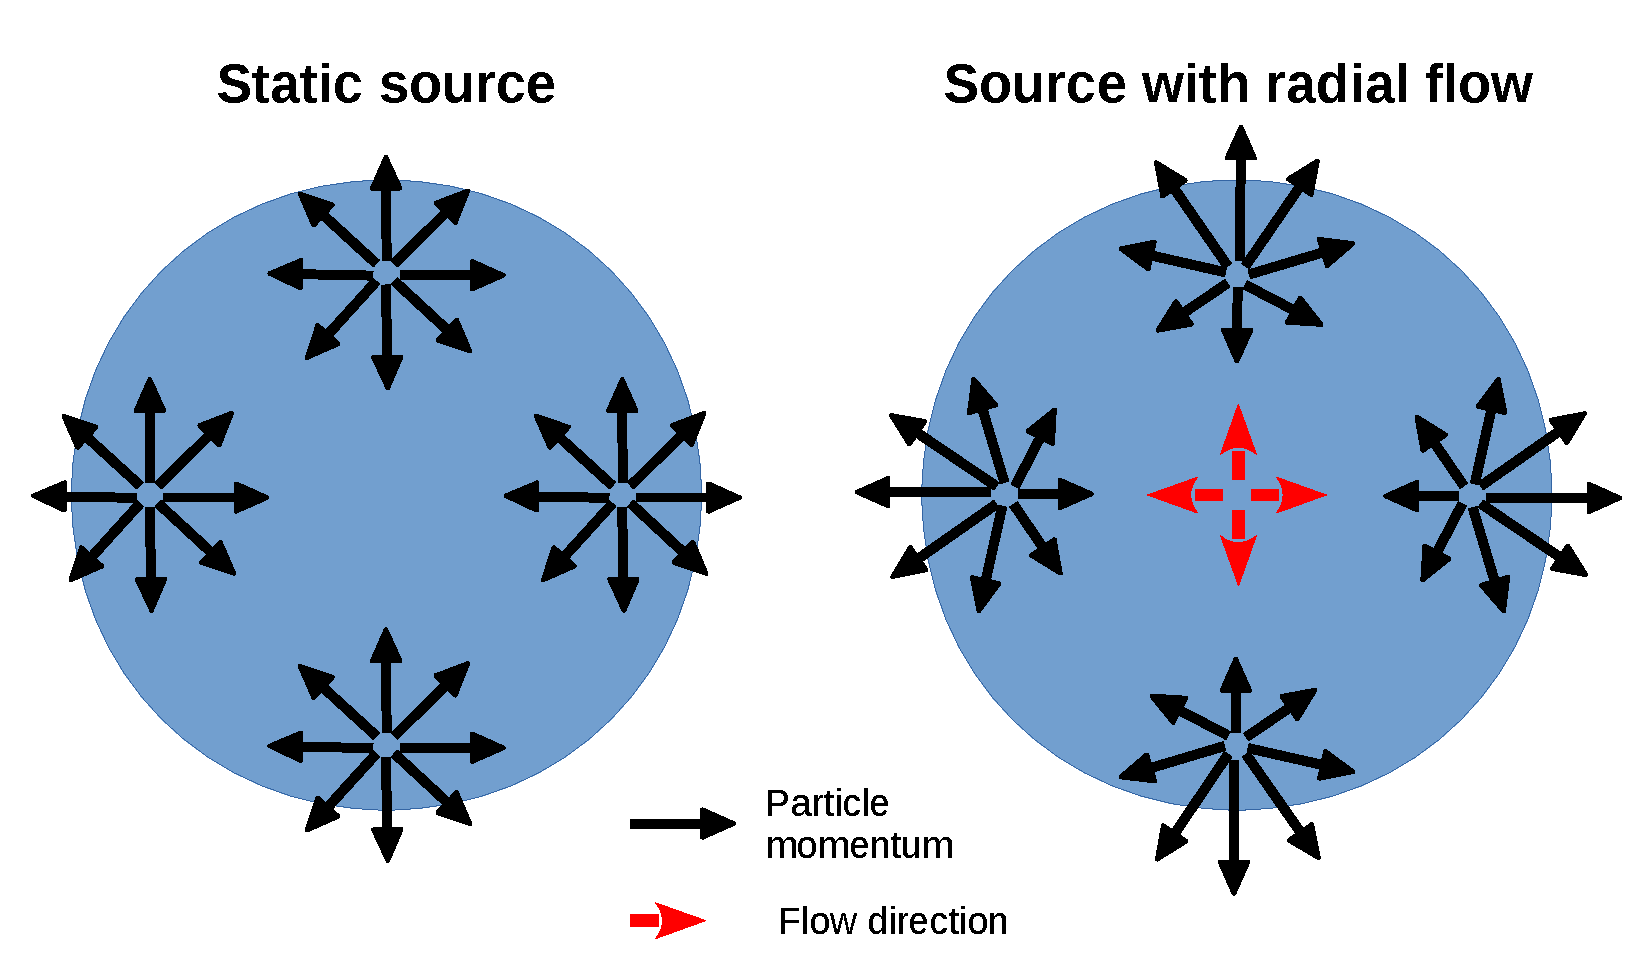
\includegraphics[width=36pc]{Figures/HomemadeFigures/FlowAndMomentum.pdf}
\caption[Effect of radial flow on momentum]{A cartoon showing possible emission momenta for particles at different places in the fireball.
(Left) In a static source where no particles interact, particles are emitted isotropically, and there are no rescatterings to change their momenta.
(Right) In an evolving source, the pressure of the fireball creates an outward radial flow of particles.
Particles are more likely to be emitted with their momenta pointing outward.}
\label{fig:FlowAndMomentum}
\end{figure}

\begin{figure}[hbt]
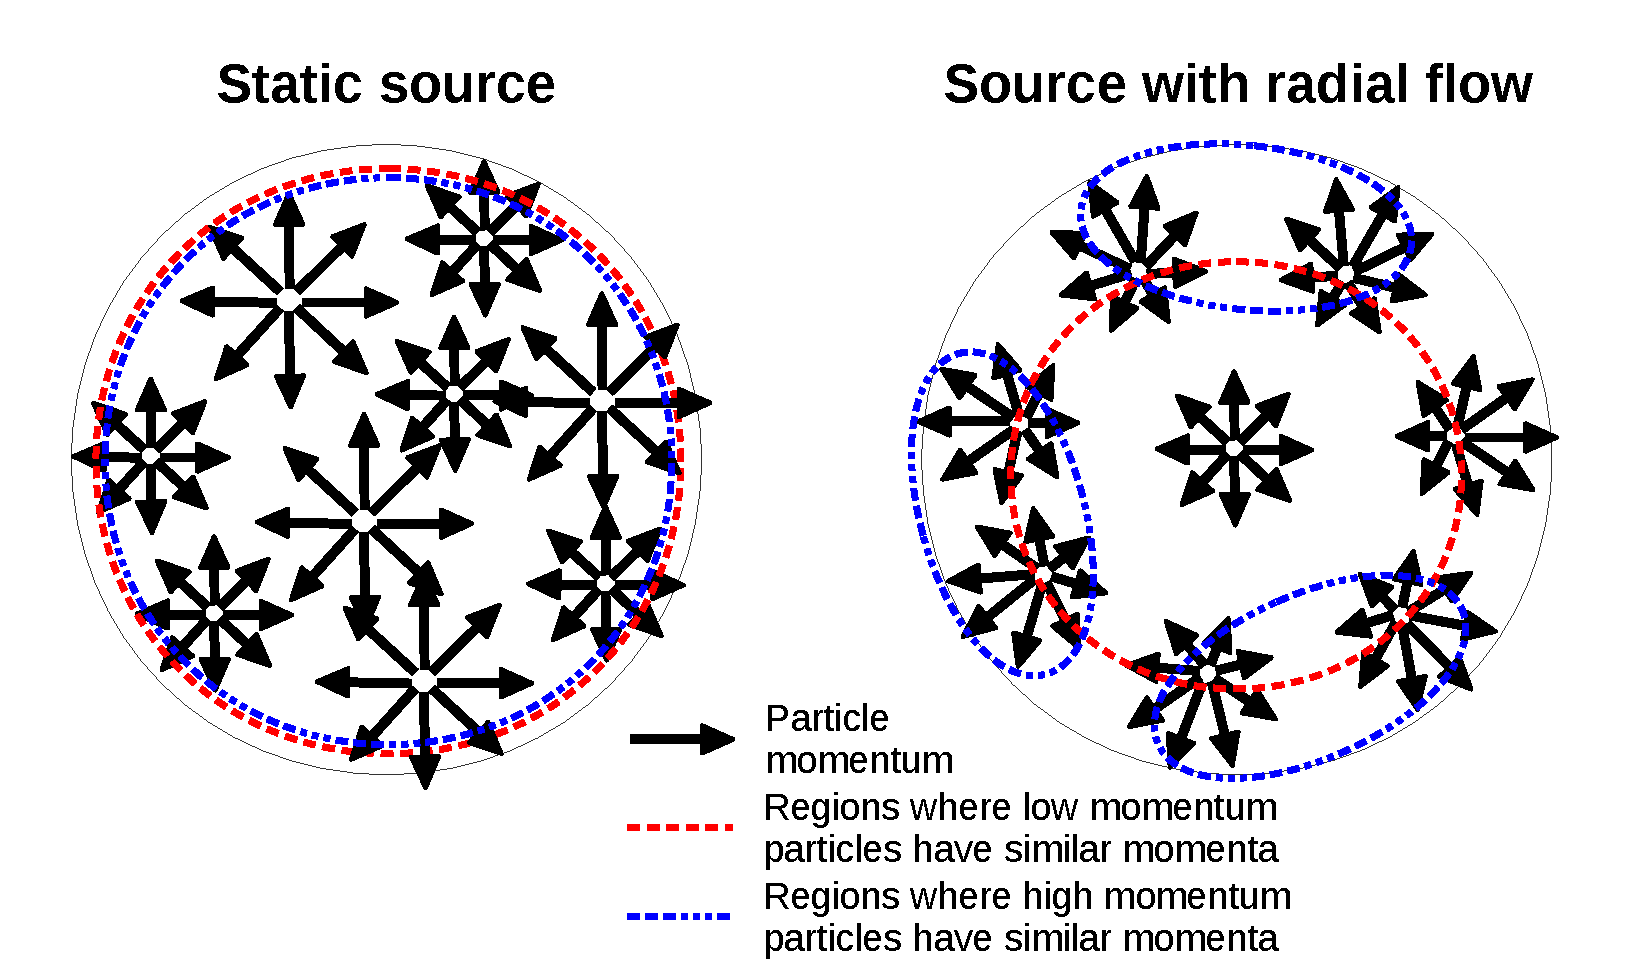
\includegraphics[width=36pc]{Figures/HomemadeFigures/RegionsOfHomogeneity.pdf}
\caption[Regions of homogeneity]{A cartoon showing regions of homogeneity---the regions where particles can be found with similar momenta and thus small relative momentum $k^* = \sqrt{-(p_1 - p_2)^2}/2$.
(Left) In a static source where no particles interact, particles are emitted isotropically throughout the interaction region.
Pairs of high momentum particles with small $k^*$ can be found throughout the fireball, as can pairs of low momentum particles with small $k^*$.
The regions of homogeneity are essentially the size of the fireball for pairs of any momentum.
(Right) In an evolving source, the pressure of the fireball boosts the momenta of particles outward.
High momentum particles with small $k^*$ are only found close together in small regions.
Low momentum particles with small $k^*$ can be found in larger regions.
High momentum particles have small regions of homogeneity, while low momentum particles have medium-sized regions.}
\label{fig:RegionsOfHomogeneity}
\end{figure}


Femtoscopic analyses traditionally study pions \cite{Goldhaber:1960sf,Aamodt:2011mr} because of their ready availability.  
However, measurements of heavier particles such as kaons \cite{Abelev:2012ms} and baryons \cite{Gos:2007cj} can serve to complement the pion results.  
One motivation for studying an assortment of heavier particles is to test the hydrodynamic prediction that radial flow should cause the source radii to scale roughly as the inverse of the transverse mass $1/m_{\mathrm{T}} = (m^2 + k^2_T)^{-1/2}$ of the particles \cite{Csorgo:1995bi,Lisa:2005dd}, where $m$ is the particle mass and $k_T$ is the transverse momentum of the particle.
An example of this can be seen in Figure \ref{fig:RegionsOfHomogeneity}.
On the left we see a fireball with no interactions between particles and thus no flow.
The collision of the heavy-ions created particles thermally (a spectrum of low to high momentum), and isotropically (in terms of where the particles were created, and direction of their momentum upon creation).
With no rescattering, their final momenta are the same as their initial momenta.
Therefore, when one looks for a region of homogeneity, the region where pairs of particles can be found with $k^* \approx 0$, one sees that it is essentially the entirety of the fireball.
This is the case both for low momentum particles and high momentum particles.
On the right side of Figure \ref{fig:RegionsOfHomogeneity}, we see an expanding fireball.
Because of the internal pressure of the fireball, outward travelling particles tend to have a large momentum and inward particles a small momentum.
Now when one looks for regions of homogeneity, one sees different results for large and small momentum particles.
For two particles with large momentum to have $k^* \approx 0$, they need to be on the same "side" of the fireball.
The dashed blue lines represent these regions of homogeneity.
For this simple case of a circular fireball, the blue circled regions are all about the same size.
Here, one would say that the overall homogeneity region for large momentum particles is small.
In contrast, the small momentum particles have a larger region of homogeneity.
Inward-traveling particles from near the edge have approximately the same momentum as outward traveling particles in the center (both pointing the same direction).
Even particles traveling in opposite directions still have a fairly small $k^*$.
So these low momentum particles have a larger homogeneity region than the high-momentum particles, but even so their region is not the size of the entire fireball.

Femtoscopy can measure homogeneity regions.
In doing so, it yields a snapshot of the final size and shape of the interaction region.
While it isn't a complete picture of the fireball, it is nonetheless the best picture experimentally available.

\subsection{Hadronic interactions}
\label{sec:HadronicInteractions}


Femtoscopic correlation functions are sensitive to the interactions between the particles.
For identical, charged pion analyses, the quantum interference effects and large Coulomb interactions drown out the interactions of the strong nuclear force.
However, for pairs of particles such as protons (pp) or neutral kaons ($K^0_\mathrm{s}K^0_\mathrm{s}$), the strong interactions are significant.
%Those interactions can be accounted for in the two-particle wave function, often with a simple s-wave scattering approximation.
As we will discuss in Section \ref{sec:WaveFunction}, these interactions are taken into account via the two-particle wave function.
For some pairs of particles, the strength and range of their interaction is well known. For example, decades of experiments have provided a wealth of pp scattering information \cite{Perez:2013jpa}.
While there are some predictions for hadron scattering lengths coming from chiral perturbation theory \cite{Mai:2009ce}, there are many hadron-hadron pairs for which little to no experimental data is available. And the interactions of hadron-antihadron pairs have been explored even less.

More information on these interactions can improve several disparate areas of research, including rescattering calculations used in modeling the evolution of heavy-ion collisions \cite{Bleicher:1999xi}; binding energy models used in hypernuclear structure theory \cite{Hiyama:2002yj,Filikhin:2002wm}; and, in the case of the lambda baryon ($\Lambda$), the equations of state which describe the properties of neutron stars \cite{SchaffnerBielich:2008kb,Wang:2010gr}.

One place where the absence of scattering information is relevant is with the Ultrarelativistic Quantum Molecular Dynamics model (UrQMD) \cite{Bleicher:1999xi}. UrQMD simulates particle creation and subsequent evolution in heavy-ion collisions.
It is also used in conjunction with other heavy-ion collision models \cite{Bass:2000ib,Ryu:2012at,Song:2013qma}; those models simulate the early- and mid-stage qualities of events via macroscopic transport models such as hydrodynamics, and then use UrQMD to handle the late hadronic stage of the collisions.
UrQMD calculates the positions and momenta of particles at fixed time steps, and it uses known particle cross-sections to determine how particles scatter off each other.
If no experimental cross-section data is available for collisions of a particular pair of hadrons, then UrQMD extrapolates from known data.
In the case of baryon-antibaryon pairs, the annihilation cross-sections at a given center of mass energy $\sqrt{s}$ are all treated as having the same annihilation cross-section as proton-antiproton pairs at the same $\sqrt{s}$.
Femtoscopy gives us a tool with which to measure these interactions so as to improve the accuracy of future rescattering models.

There have been several recent femtoscopy success stories at the Relativistic Heavy Ion Collider (RHIC) from the STAR Experiment (Solenoidal Tracker at RHIC).
In one study of $\bar{\mathrm{p}}\bar{\mathrm{p}}$ pairs, STAR measured the s-wave scattering parameters of $\bar{\mathrm{p}}\bar{\mathrm{p}}$, and found that they are consistent with those of pp \cite{Adamczyk:2015hza}.
In another study, STAR saw unexpected differences between the measured femtoscopic radii of p$\Lambda$ and p$\bar{\Lambda}$ pairs, with the latter pairs being about a factor of two smaller \cite{Adams:2005ws}.
A reanalysis of that data implemented a new method for accounting for signal contaminations in the correlation functions \cite{Kisiel:2014mma}.
Rather than correct for impurity with a simple scaling factor, the new method attempted to quantify the effect of the residual correlations (the femtoscopic correlations arising from the contaminations).
With the new method in place, the extracted $p\bar{\Lambda}$ radius was consistent with the $p\Lambda$ radius ($R_{\mathrm{p}\bar{\Lambda}} = 2.83 \pm 0.12$ fm vs.\ $R_{\mathrm{p}\Lambda} = 3.09 \pm 0.3^{+0.17}_{-0.25} \pm 0.2$ fm).
The analysis presented in this thesis, $\Lambda\Lambda$ and $\Lambda\bar{\Lambda}$ femtoscopy, uses this approach for handling residual correlations; the details can be found in Sections \ref{sec:Residual} and \ref{sec:LambdaParams}.


\subsection{$\Lambda$ femtoscopy}
\label{sec:LambdaFemto}

\begin{figure}[hbt]
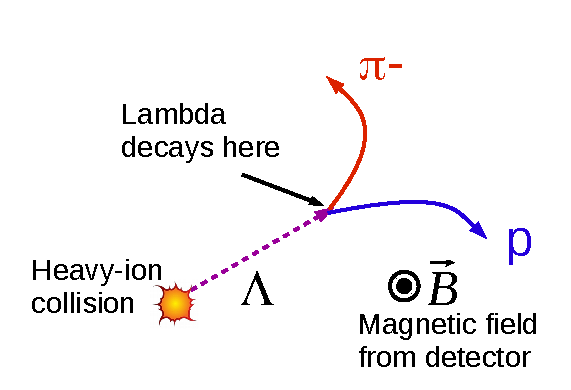
\includegraphics[width=36pc]{Figures/HomemadeFigures/LambdaDecayCartoon.pdf}
\caption[Cartoon of lambda decay]
{
Cartoon of the decay of a lambda baryon ($\Lambda$).
A $\Lambda$ moving near the speed of light decays into a proton and a pion after traveling a few centimeters away from the fireball in which it was created. 
The $\Lambda$ is charge-neutral, so it is not detected directly; instead it is reconstructed by looking for pairs of charged particles that fit a certain decay topology.
See Section \ref{sec:ParticleSelection} for more details about $\Lambda$ reconstruction.
%The $\Lambda$ is charge-neutral, so its trajectory is straight.
%But the proton and pion that it decays into are charged, so their trajector is curved by the magnetic field created by the surrounding detector.
}
\label{fig:LambdaDecayCartoon}
\end{figure}

% Describe why lambdas are useful for these studies
The frontier of femtoscopy lies in studying heavier particle pairs.
% Radii affected by freezeout times, 
By virtue of their larger mass, particles such as p, $\Lambda$, and the cascade baryons ($\Xi^-$ and $\Xi^0$) can yield femtoscopic radii at much larger $m_\mathrm{T}$ than are accessible via pions.
In addition, femtoscopy gives access to the scattering paramaters of these particles, information that is sorely needed for a number of heavier particle pairs.
Finally, the process of identifying V0s, neutral particles such as $\Lambda$ and $K^0_\mathrm{s}$ whose decay into charged particles looks roughly "V"-shaped, differs significantly from the process of identifying charged particles.
Figure \ref{fig:LambdaDecayCartoon} shows a cartoon of a $\Lambda$ decay.
Because of the differences in their analysis techniques, V0 particle femtoscopy and charged particle femtoscopy can therfore provide useful consistency checks for each other, as seen in the recent charged and neutral kaon analyses at ALICE \cite{Adam:2015vja}.

As mentioned above, there is a need for experimental study of exotic particle interactions.
For example, there is a sizable disparity in the p$\Lambda$ singlet-state scattering length $f_0$ between the leading order ($f_0 = 1.9$ fm) and next-to-leading order ($f_0 = 2.9$ fm) chiral effective field theory calculations \cite{Haidenbauer:2013oca}.
%Scattering data for the short-lived (<lifetime> \cite{Olive:2016xmw}) , neutral $\Lambda$ are hard to come by.
There are only a handful of measurements of the $\Lambda\Lambda$ scattering length: one via the decay of a hypernucleus (a nucleus which contains one or more strange particles) \cite{Takahashi:2001nm,Filikhin:2002wm,Hiyama:2002yj}, and one via femtoscopy at STAR \cite{Adamczyk:2014vca}, and another via femtoscopy at the Super Proton Synchrotron (SPS) \cite{Andersen:1999gq}.
The SPS experiment did not have enough data to resolve any nuclear interaction.
The other results are inconsistent with each other --- their scattering lengths differ in sign, tantamount to a difference between attractive and repulsive interactions --- so further measurements are necessary.

Research on $\Lambda$ particles is statistically quite demanding compared to similar research on pions.
In $\sqrt{s_{\mathrm{NN}}}=2.76$ TeV central Pb-Pb collisions at the LHC, there are about 4 $\Lambda$ created per 100 $\pi$ \cite{Zhang:2013fta}.
Nonetheless, modern particle colliders, including RHIC and the LHC, are in a unique position to perform $\Lambda$ femtoscopy.
At the LHC, Pb-Pb collisions at $\sqrt{s_{\mathrm{NN}}}=2.76$ TeV have mid-rapidity $\Lambda$ yields $\sim 2.5$ times larger than those measured in the aforementioned fixed-target SPS experiment, which had Pb-Pb collisions with a beam energy $E = 158$ A GeV ($\sqrt{s_{\mathrm{NN}}} \approx 17.3$ GeV)  \cite{Abelev:2013xaa,Alt:2008qm}.
But the relevant quantity for femtoscopy is number of pairs, not number of particles, so the 2.5 times increase in particles leads to about 6 times more pairs. 
Moreover, at the LHC, the baryochemical potential $\mu_\mathrm{b} \approx 0$ MeV \cite{Stachel:2013zma}, meaning that the ratio of baryons to antibaryons is unity.
Therefore, the statistics for $\bar{\Lambda}$ analyses should be comparable to those for $\Lambda$ analyses.


%There, $\Lambda$ yields are high enough to get enough data
%The $\Lambda$ has a mass of $\sim$1116 MeV$/c^2$, almost 1000 MeV more than a $\pi$, and about 180 MeV$/c^2$ heavier than a proton.
%Compared to $\pi$, the production of $\Lambda$ in collisions is signficantly suppressed by mass alone.

% At lower energies, strangeness suppression also results in lower lambda yields. Describe strangeness suppression.


Several physics effects can be seen in $\Lambda$ and $\bar{\Lambda}$ correlation functions.
The primary effect seen in $\Lambda\bar{\Lambda}$ correlations should be the final state interactions (FSI) of the strong nuclear force.  
There should be a depletion of baryon-antibaryon pairs at low relative momentum due to annihilation channels.
Suppressions of this sort have been seen in $p \bar{p}$ interactions \cite{Gos:2007cj,Adamczyk:2015hza}, though FSI effects in charged particle studies are somewhat obfuscated by Coulomb effects.  
$\Lambda\Lambda$ and $\bar{\Lambda}\bar{\Lambda}$ correlation functions are expected to be consistent with each other.
In addition to FSI effects, they will also have a suppression at low relative momentum due to Fermi-Dirac quantum interference.
The primary goal of this analysis is to extract the FSI scattering parameters of these pairs, as well as their femtoscopic radii.

%It should also be noted that the H-dibaryon may have two $\Lambda$ as one of its decay channels \cite{PhysRevLett.38.195}, though a recent study at ALICE has suggested that a $\Lambda\Lambda$ bound state is unlikely \cite{...}.  

In this thesis, we present $\Lambda$ and $\bar{\Lambda}$ femtoscopy from $\sqrt{s_{NN}}=2.76$ TeV Pb-Pb collisions measured at the LHC by ALICE.
In Chapter \ref{sec:DataMeasurement}, we discuss the experimental details involved in measuring $\Lambda$ and constructing femtoscopic correlation functions.
Chapter \ref{sec:DataAnalysis} describes how we analyzed the correlation functions.
This includes a discussion of the theoretical formalism used to fit the data (Section \ref{sec:CorrelationFunctionModel}), an account of how we treat signal contaminations (Sections \ref{sec:Residual}--\ref{sec:MomResCorrectFit}), a walkthrough of our fit procedure (Section \ref{sec:FitProcedure}), and a breakdown of our extracted scattering parameters and radii (Section \ref{sec:FitResults}).





